\chapter{Results}
\label{ch:results}

\section{Testing}
The graphs used during testing was either created randomly or created manually, the random graphs had 40 nodes in it, 10 lethal and 2 exit nodes. In the manually created graph we had 8 nodes, with 2 lethal and 1 exit node. The test started with using 1 ant in the AntSystem, and compared it to brute force and random. This was done 100 times where the lethal nodes was changed each time. If the AntSystem did not find an solution for the node, random was used for the humans to represent that it had to guess its way to an exit. The next step was to do the same again with 2 ants in the AntSystem, this continued to 100 ants. This was to see how well the AntSystem did with more ants and to see if and where it became just as good as brute force.

There is a clear difference on how much time the simulation needed for both our crated graphs. As the the bigger graph used a lot more time with brute force then the smaller one did. This was to be expected as brute force will need more and more resources as it have a bigger environment to explore.

\newpage

\section{Empirical results from stimulation}

When ACO do not have many ants to explore the enviorment to find the possible paths, ACO will not do much better then random, as shown in the figures. However when ACO get to use more ants to find possible solutions to the problem, it gets better and better and goes towards brute force. When looking at absolute survivors, shown in figure \ref{fig:Rbiggraph} and figure \ref{fig:Rsmallgraph}, ACO gets the same number of survivors as brute force. However when you look at figure \ref{fig:Rsmallgraphf} ACO never reaches the same amount as brute force, only gets closer and closer to the same value. The reason for this is that on occasion in its 100 runs where the lethal nodes change, the solution for that particular scenario is hard to solve. Then ACO needs more ants to solve that particular scenario, and therefore gets better and better with more ants.

The main difference from 8 to 40 nodes is that it requires more ants to solve the problem in bigger graphs, however it is not a huge increase. This can be shown in figure \ref{fig:Rsmallgraph} and figure \ref{fig:Rbiggraph}. There is also an increase of needed ants when more lethal nodes are added to the graph, in figure \ref{fig:Rbiggraph2f} ACO get close to brute force when ACO gets to use 20 ants or more, however when more lethal nodes are added shown in figure \ref{fig:Rbiggraph5f}, ACO needs more then 30 ants to get close to brute force, and is still not as good as ACO in figure \ref{fig:Rbiggraph2f}. This is to be expected as more lethal nodes makes more likely for the ants to stumble upon them.

 Also, there is a difference when measuring absolute survivors and average survivors, in figure \ref{fig:Rsmallgraph} ACO reaches the same results as brute force, only to miss the target a few times, however in figure \ref{fig:Rsmallgraphf} ACO never reaches the exact same value, however is getting closer and closer as more ants are used in ACO.


\begin{figure} % "placement and width parameter for the width of the image space.
\hspace*{-1.5 cm}
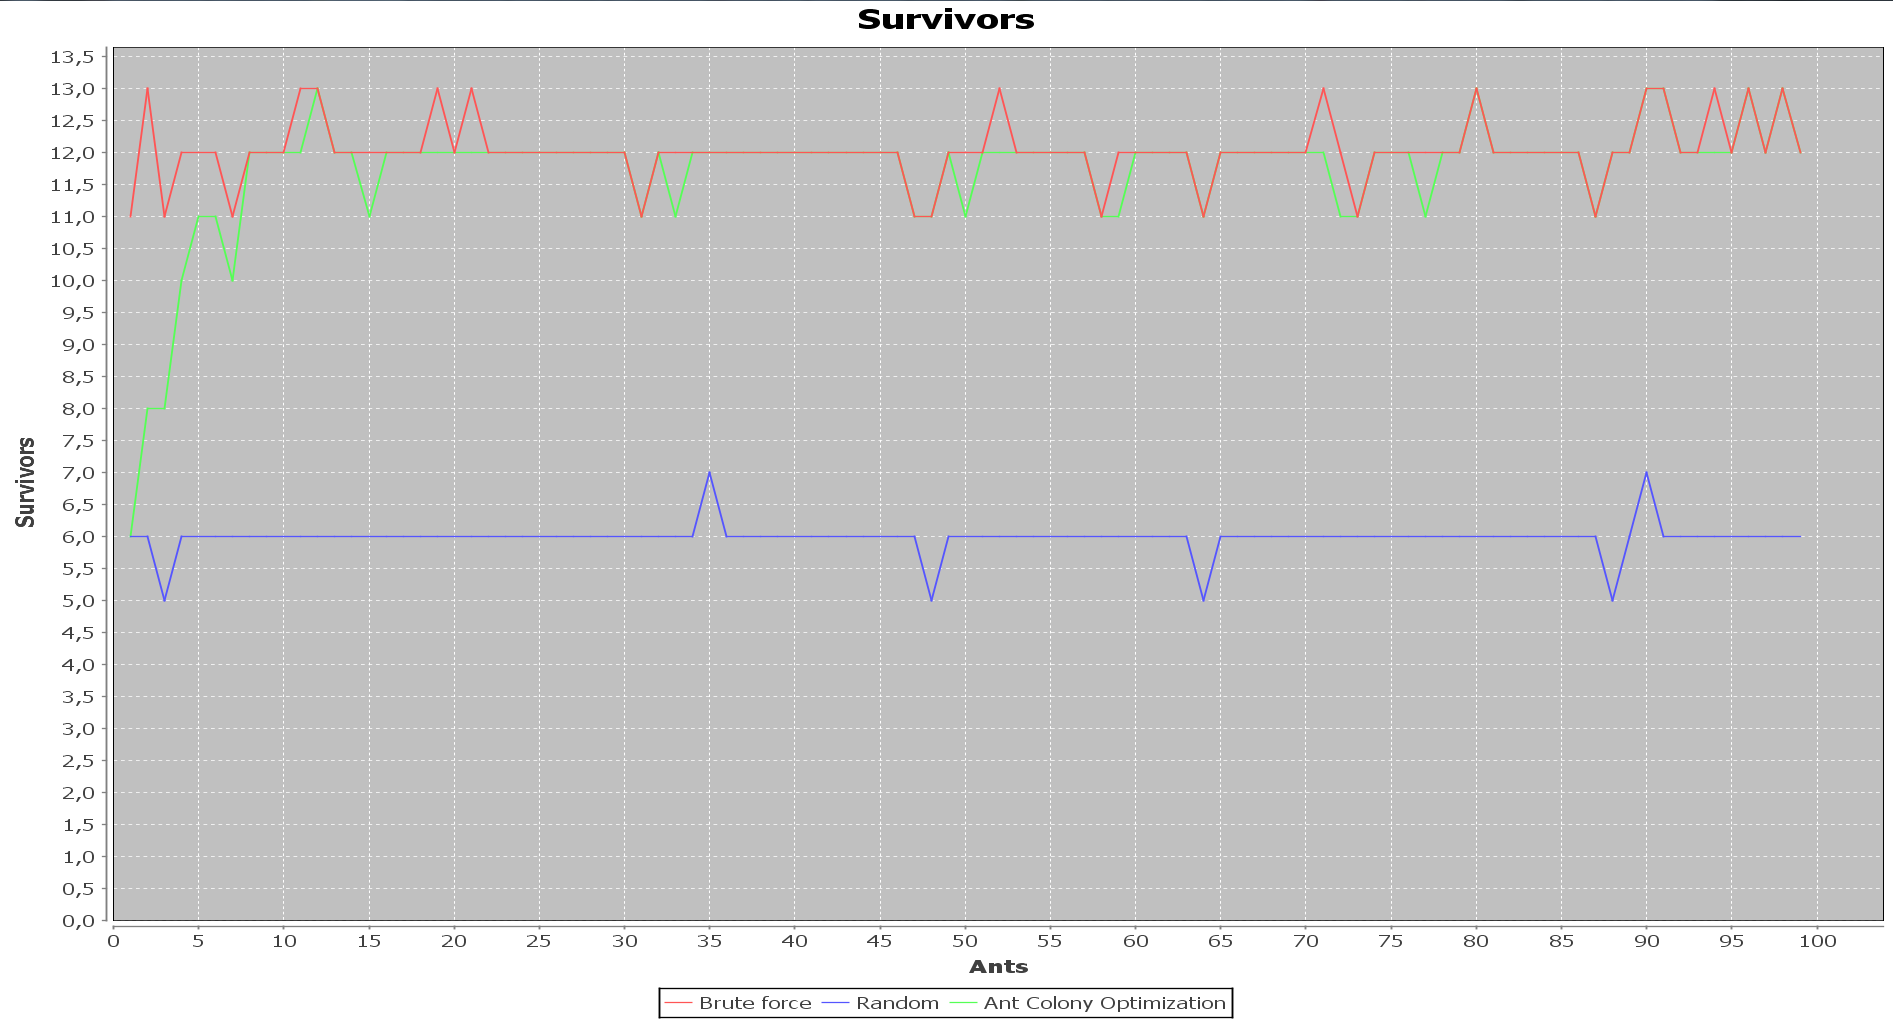
\includegraphics[width=160mm]{images/8Nodes2Leathal1Exit.png}
\caption{\textit{Graph with 8 nodes, where 2 are lethal and there is 1 exit.}}
\label{fig:Rsmallgraph}
\end{figure}

\begin{figure} % "placement and width parameter for the width of the image space.
\hspace*{-1.5 cm}
\includegraphics[width=160mm]{images/40Nodes2Leathal2Exit.png}
\caption{\textit{Graph with 40 nodes, where 2 are lethal and there is 1 exit.}}
\label{fig:Rbiggraph}
\end{figure}

\begin{figure} % "placement and width parameter for the width of the image space.
\hspace*{-1.5 cm}
\includegraphics[width=160mm]{images/Float8Nodes2Leathal1Exitpng.png}
\caption{\textit{Same as figure \ref{fig:Rsmallgraph}, however this is not absolute survivors.}}
\label{fig:Rsmallgraphf}
\end{figure}

\begin{figure} % "placement and width parameter for the width of the image space.
\hspace*{-1.5 cm}
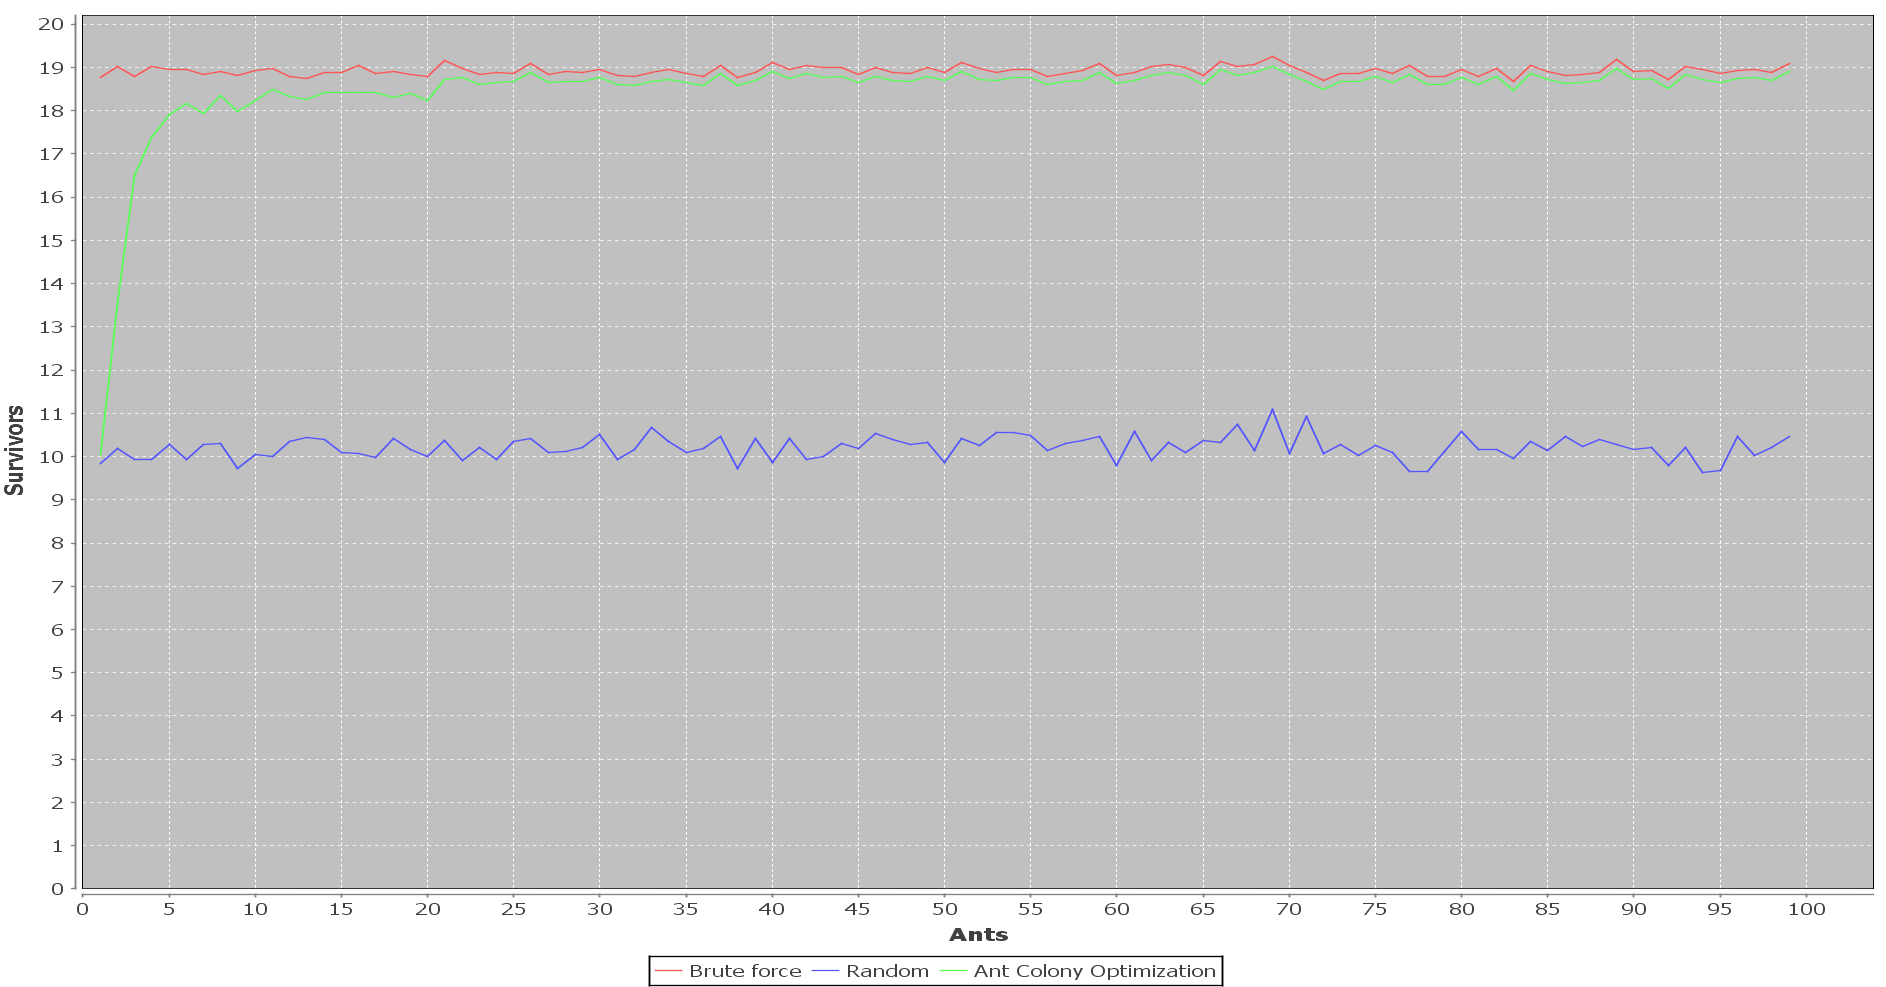
\includegraphics[width=160mm]{images/Float40Nodes2Leathal2Exit.png}
\caption{\textit{Same as figure \ref{fig:Rbiggraph}, however this is not absolute survivors.}}
\label{fig:Rbiggraph2f}
\end{figure}


\begin{figure} % "placement and width parameter for the width of the image space.
\hspace*{-1.5 cm}
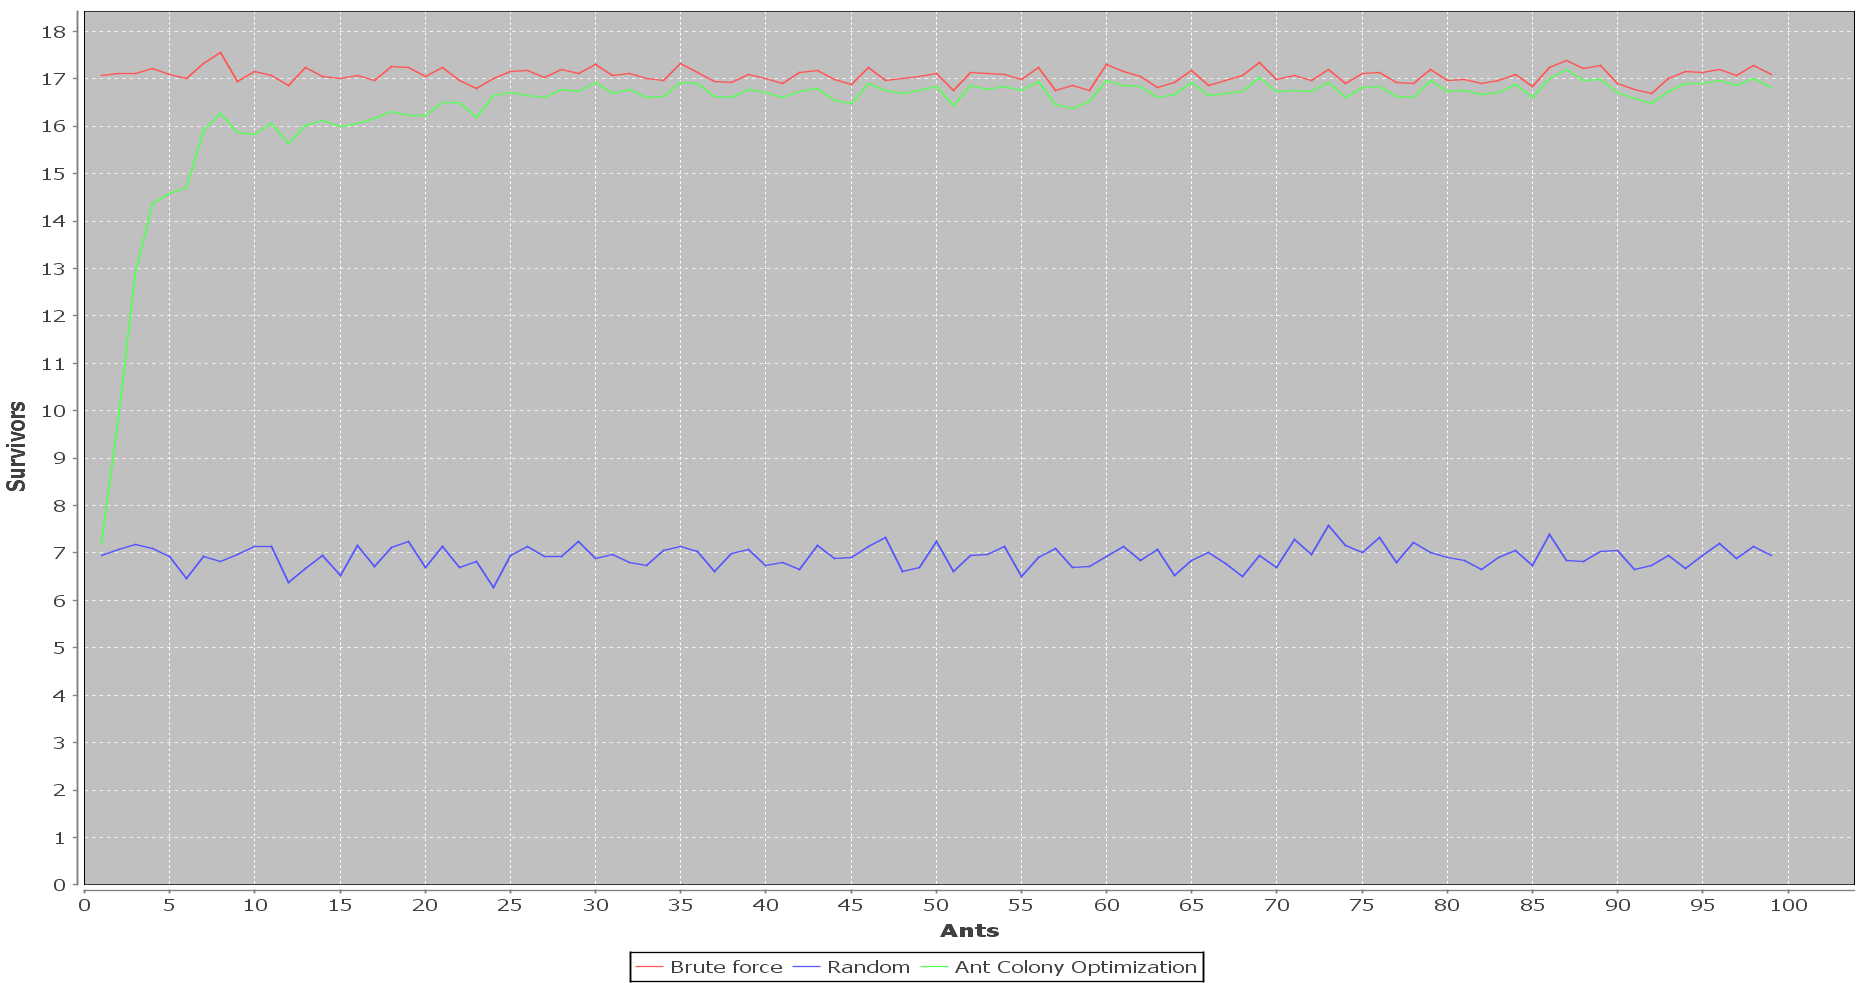
\includegraphics[width=160mm]{images/Float40Nodes5Leathal2Exit.png}
\caption{\textit{Same as figure \ref{fig:Rbiggraph2f}, only with 5 lethal nodes}}
\label{fig:Rbiggraph5f}
\end{figure}
\pagebreak


ACO is not affected much by changing the lethal nodes after each turn, neither are random or brute force for that matter too. This is shown in the fact that they all ho up and down at at the same time. The only exception to this is when ACO only uses a few ants, as it gets better and better by using more ants to find solutions. This is a good thing as the next step is creating hazards that are dynamic and not stationary as this will be a bigger challenge for the AntSystem to solve. 





%\includegraphics[width=150mm]{Float8Nodes2Leathal1Exitpng.png}
%\includegraphics[width=150mm]{40Nodes2Leathal2Exit.png}